\chapter{Martingales}
\section{Lecture 3}

The $\sigma$-algebra can change since we gain more information over time.

\begin{definition}[Filtration]
Let $(\Omega,\mcal{F},\Prob)$ be a probability space. A
\emph{filtration} is a nondecreasing family
$\{\mcal{F}_t\}_{t\geq 0}$ of sub-$\sigma$-algebras of $\mcal{F}$.
\end{definition}

Intuitively, $\mcal{F}_t$ represents all information available by time
$t$. We define
\[
    \mcal{F}_\infty
    = \sigma\left(\bigcup_{t\geq 0}\mcal{F}_t\right).
\]

Let $\{X_t\}_{t\geq 0}$ be a stochastic process. The filtration
\emph{generated} by $\{X_t\}$ is
\[
    \mcal{F}_t^X = \sigma(X_s:0\leq s\leq t),
    \qquad 0\leq t<\infty.
\]

\begin{definition}[Adapted Process]
A process $\{X_t\}_{t\geq 0}$ is \emph{adapted} to a filtration
$\{\mcal{F}_t\}_{t\geq 0}$ if $X_t$ is $\mcal{F}_t$-measurable for
every $t\geq 0$.
\end{definition}

The filtration generated by $\{X_t\}$ is the smallest filtration to
which $\{X_t\}$ is adapted.

\begin{definition}[Usual Conditions for Filtrations]
A filtration satisfies the \emph{usual conditions} if:

\begin{enumerate}
    \item[(i)] it is right-continuous:
    \[
        \mcal{F}_t
        = \mcal{F}_{t+}
        := \bigcap_{s>t}\mcal{F}_s;
    \]

    \item[(ii)] it is complete: $\mcal{F}_0$ contains every subset of
    every $\Prob$-null set in $\mcal{F}$.
\end{enumerate}
\end{definition}

Right continuity says that information which is available at every time
immediately after $t$ is already available at time $t$. It does
\emph{not} say that information cannot arrive at $t$ itself. In fact,
left continuity would be unnatural in most models: for example,
$B_t$ is known at time $t$ in the Brownian filtration, but it cannot in
general be determined from observations strictly before $t$.

\subsection*{Martingale Theory}

\begin{definition}[Stopping Time]
Given a filtered probability space
$(\Omega,\mcal{F},\{\mcal{F}_t\}_{t\geq 0},\Prob)$, an
$[0,\infty]$-valued random variable $T$ is a \emph{stopping time} if
\[
    \{T\leq t\}\in\mcal{F}_t
    \qquad \text{for every }t\geq 0.
\]
\end{definition}

The interpretation is: by time $t$, one can determine whether stopping
has already occurred.

\begin{proposition}[Hitting times of continuous processes]
Suppose that $X$ is adapted and has continuous sample paths. For
$a\in\mathbb{R}$, define
\[
    T_a(\omega)
    = \inf\{s\geq 0:X_s(\omega)=a\},
\]
where the infimum of the empty set is $\infty$. Then $T_a$ is a
stopping time.
\end{proposition}

\begin{proof}
Fix $t\geq 0$. Since $X$ is adapted, $X_q$ is
$\mcal{F}_q$-measurable, hence $\mcal{F}_t$-measurable, for every
$q\in\mathbb{Q}\cap[0,t]$. Thus
\[
    Y_t
    := \inf_{q\in\mathbb{Q}\cap[0,t]} |X_q-a|
\]
is $\mcal{F}_t$-measurable.

We claim that
\[
    \{T_a\leq t\}=\{Y_t=0\}.
\]
If $T_a\leq t$, continuity gives a time $s\in[0,t]$ with $X_s=a$.
Choosing rational $q$'s approaching $s$ and using continuity gives
$Y_t=0$.

Conversely, if $Y_t=0$, choose $q_n\in\mathbb{Q}\cap[0,t]$ such that
$|X_{q_n}-a|\to 0$. By compactness of $[0,t]$, some subsequence
$q_{n_j}$ converges to $s\in[0,t]$. Continuity gives
\[
    X_s=\lim_{j\to\infty}X_{q_{n_j}}=a,
\]
so $T_a\leq t$. Therefore
\[
    \{T_a\leq t\}=\{Y_t=0\}\in\mcal{F}_t.
\]
\end{proof}

Continuity is sufficient because it lets us recover whether the path
has hit $a$ by time $t$ from its values at rational times up to $t$.
Adaptedness alone is not enough for this particular argument.

In contrast, a last hitting time need not be a stopping time because determining whether a visit was the last one generally requires knowledge of the future.
\begin{example}[A last visit time need not be a stopping time]
Let $\xi_1,\xi_2$ be independent random variables satisfying
\[
    \Prob(\xi_i=1)=\Prob(\xi_i=-1)=\frac12.
\]
Define the simple random walk
\[
    X_0=0,\qquad X_1=\xi_1,\qquad X_2=\xi_1+\xi_2,
\]
with its natural filtration
\[
    \mcal F_n=\sigma(\xi_1,\ldots,\xi_n),
    \qquad n=1,2,
\]
and $\mcal F_0=\{\varnothing,\Omega\}$.

Let
\[
    L=\max\{n\in\{0,1,2\}:X_n=0\}
\]
be the last time the random walk visits $0$ before time $2$.
Then $L$ is not a stopping time with respect to
$\{\mcal F_n\}_{n=0}^2$.
\end{example}

\begin{proof}
We show that $\{L\leq 1\}\notin\mcal F_1$.

Since $X_1\in\{-1,1\}$, the random walk cannot be at $0$
at time $1$. Thus,
\[
    \{L\leq 1\}
    =\{X_2\neq 0\}
    =\{\xi_1=\xi_2\}.
\]

Now, $\mcal F_1=\sigma(\xi_1)$, so the information
available at time $1$ consists only of the value of $\xi_1$.

However, knowing $\xi_1$ does not determine whether
$\xi_1=\xi_2$. For instance, the outcomes
\[
    (\xi_1,\xi_2)=(1,1)
    \qquad\text{and}\qquad
    (\xi_1,\xi_2)=(1,-1)
\]
are indistinguishable at time $1$, yet the former belongs
to $\{L\leq 1\}$ while the latter does not.

More formally, the sigma-algebra $\mcal F_1$ consists of
\[
    \mcal F_1
    =\{\varnothing,\Omega,\{\xi_1=1\},\{\xi_1=-1\}\}.
\]
Since $\{\xi_1=\xi_2\}$ is not one of these events,
\[
    \{L\leq 1\}\notin\mcal F_1.
\]

Therefore, $L$ is not a stopping time.
\end{proof}

As a general principle, all buying and selling times should be stopping
times: a strategy may use present and past information, but not future
information.

\begin{proposition}
If $S$ and $T$ are stopping times, then $S\wedge T$, $S\vee T$, and
$S+T$ are stopping times, assuming the filtration is right-continuous.
\end{proposition}

\begin{proof}
For $t\geq 0$,
\[
    \{S\wedge T\leq t\}
    =
    \{S\leq t\}\cup\{T\leq t\}\in\mcal{F}_t,
\]
and
\[
    \{S\vee T\leq t\}
    =
    \{S\leq t\}\cap\{T\leq t\}\in\mcal{F}_t.
\]

For the sum, first observe that for $r>0$,
\[
    \{S+T<r\}
    =
    \bigcup_{q\in\mathbb{Q}\cap(0,r)}
    \bigl(\{S<q\}\cap\{T<r-q\}\bigr).
\]
Each event on the right belongs to $\mcal{F}_r$, so
$\{S+T<r\}\in\mcal{F}_r$. Therefore,
\[
    \{S+T\leq t\}
    =
    \bigcap_{n=1}^\infty
    \left\{S+T<t+\frac{1}{n}\right\}
    \in
    \bigcap_{n=1}^\infty\mcal{F}_{t+1/n}
    =
    \mcal{F}_{t+}
    =
    \mcal{F}_t.
\]
Thus $S+T$ is a stopping time.
\end{proof}

\begin{definition}[$\sigma$-algebra at a stopping time]
Let $T$ be a stopping time. Define
\[
    \mcal{F}_T
    =
    \left\{
        A\in\mcal{F}_\infty:
        A\cap\{T\leq t\}\in\mcal{F}_t
        \text{ for every }t\geq 0
    \right\}.
\]
\end{definition}

The correct intuition is not that $A$ ``happens before $T$.'' Rather,
$A\in\mcal{F}_T$ means that $A$ is \emph{knowable by time $T$}: on the
event $\{T\leq t\}$, one can determine by time $t$ whether $A$
occurred.

\begin{proposition}
$\mcal{F}_T$ is a $\sigma$-algebra.
\end{proposition}

\begin{proof}
Since $T$ is a stopping time,
\[
    \Omega\cap\{T\leq t\}=\{T\leq t\}\in\mcal{F}_t,
\]
so $\Omega\in\mcal{F}_T$.

If $A\in\mcal{F}_T$, then
\[
    A^c\cap\{T\leq t\}
    =
    \{T\leq t\}\setminus\bigl(A\cap\{T\leq t\}\bigr)
    \in\mcal{F}_t.
\]
Thus $A^c\in\mcal{F}_T$.

Finally, if $A_1,A_2,\ldots\in\mcal{F}_T$, then
\[
    \left(\bigcup_{n=1}^\infty A_n\right)\cap\{T\leq t\}
    =
    \bigcup_{n=1}^\infty
    \left(A_n\cap\{T\leq t\}\right)
    \in\mcal{F}_t.
\]
Therefore $\bigcup_{n=1}^\infty A_n\in\mcal{F}_T$.
\end{proof}

For a process $X$ and a stopping time $T$, define the stopped process
$X^T$ by
\[
    X_t^T:=X_{t\wedge T}.
\]
Pathwise, $X^T$ follows $X$ until the random time $T$, then remains
frozen at the value $X_T$:
\[
    X_t^T(\omega)=
    \begin{cases}
        X_t(\omega), & t<T(\omega),\\
        X_{T(\omega)}(\omega), & t\geq T(\omega).
    \end{cases}
\]

\begin{definition}[Submartingales, Supermartingales, and Martingales]
Let $(\Omega,\mcal{F},\{\mcal{F}_t\},\Prob)$ be a filtered probability
space. An adapted process $\{X_t\}$ is a \emph{submartingale} if:

\begin{enumerate}
    \item[(i)] $X_t\in L^1(\Omega,\mcal{F},\Prob)$ for every $t$;
    \item[(ii)] for every $s<t$,
    \[
        \E[X_t\mid\mcal{F}_s]\geq X_s.
    \]
\end{enumerate}

If the inequality is reversed, $X$ is a \emph{supermartingale}. If
there is equality, $X$ is a \emph{martingale}.
\end{definition}

\begin{figure}[h]
\centering
%html-figure: super-sub-martingale.svg
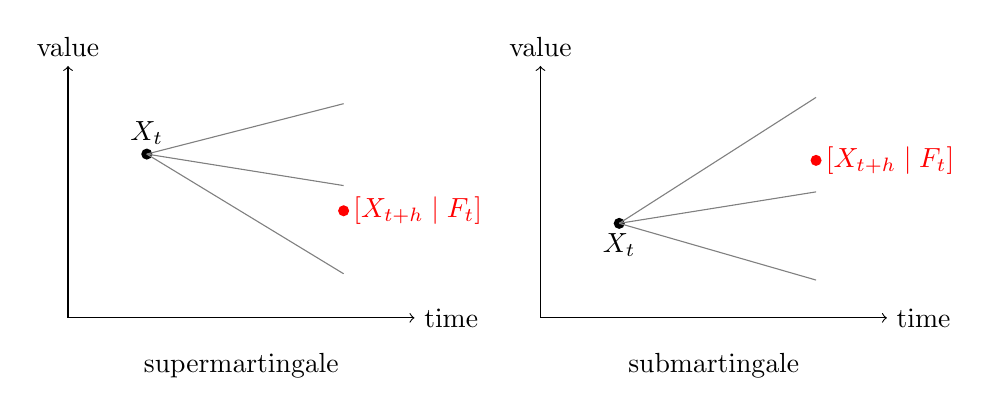
\begin{tikzpicture}[x=1cm,y=0.8cm]
    \draw[->] (0,0) -- (4.4,0) node[right] {time};
    \draw[->] (0,0) -- (0,4) node[above] {value};

    \fill (1,2.6) circle (2pt) node[above] {$X_t$};
    \draw[gray] (1,2.6) -- (3.5,3.4);
    \draw[gray] (1,2.6) -- (3.5,2.1);
    \draw[gray] (1,2.6) -- (3.5,0.7);
    \fill[red] (3.5,1.7) circle (2pt)
        node[right] {$\E[X_{t+h}\mid\mcal{F}_t]$};
    \node at (2.2,-0.75) {supermartingale};

    \begin{scope}[xshift=6cm]
        \draw[->] (0,0) -- (4.4,0) node[right] {time};
        \draw[->] (0,0) -- (0,4) node[above] {value};

        \fill (1,1.5) circle (2pt) node[below] {$X_t$};
        \draw[gray] (1,1.5) -- (3.5,0.6);
        \draw[gray] (1,1.5) -- (3.5,2.0);
        \draw[gray] (1,1.5) -- (3.5,3.5);
        \fill[red] (3.5,2.5) circle (2pt)
            node[right] {$\E[X_{t+h}\mid\mcal{F}_t]$};
        \node at (2.2,-0.75) {submartingale};
    \end{scope}
\end{tikzpicture}
\caption{A martingale condition concerns conditional averages, not the
direction of every individual sample path.}
\end{figure}


\section{Lecture 4}

\begin{definition}[Upcrossings]
Let $\{X_n\}_{n\in\mathbb{N}_0}$ be a discrete-time process, and fix
$a<b$. The number $U_N[a,b]$ of \emph{upcrossings} of $[a,b]$ by time
$N$ is the largest $k\in\mathbb{N}_0$ for which there exist integers
\[
    0\leq s_1<t_1<s_2<t_2<\cdots<s_k<t_k\leq N
\]
such that
\[
    X_{s_i}<a
    \qquad\text{and}\qquad
    X_{t_i}>b
    \qquad (i=1,\ldots,k).
\]
\end{definition}

\begin{figure}[h]
\centering
%html-figure: upcrossings.svg
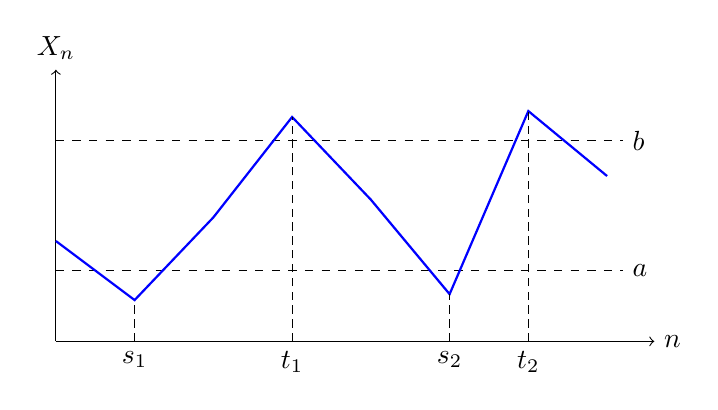
\begin{tikzpicture}[x=1cm,y=0.75cm]
    \draw[->] (0,0) -- (7.6,0) node[right] {$n$};
    \draw[->] (0,0) -- (0,4.6) node[above] {$X_n$};

    \draw[dashed] (0,1.2) -- (7.2,1.2) node[right] {$a$};
    \draw[dashed] (0,3.4) -- (7.2,3.4) node[right] {$b$};

    \draw[thick,blue]
        (0,1.7) -- (1,0.7) -- (2,2.1) -- (3,3.8)
        -- (4,2.4) -- (5,0.8) -- (6,3.9) -- (7,2.8);

    \draw[densely dashed] (1,0) -- (1,0.7);
    \draw[densely dashed] (3,0) -- (3,3.8);
    \draw[densely dashed] (5,0) -- (5,0.8);
    \draw[densely dashed] (6,0) -- (6,3.9);

    \node[below] at (1,0) {$s_1$};
    \node[below] at (3,0) {$t_1$};
    \node[below] at (5,0) {$s_2$};
    \node[below] at (6,0) {$t_2$};
\end{tikzpicture}
\caption{This path makes two upcrossings of $[a,b]$.}
\end{figure}

\begin{theorem}[Doob's Upcrossing Inequality]
Let $X$ be a supermartingale. Then
\[
    (b-a)\E[U_N[a,b]]
    \leq
    \E[(X_N-a)^-],
\]
where $x^-:=\max\{-x,0\}$.
\end{theorem}

\begin{definition}[Predictable / Previsible Process]
A discrete-time process $C=\{C_n\}_{n\geq 1}$ is
\emph{predictable} if $C_n$ is $\mcal{F}_{n-1}$ measurable for all $n \ge 1$.
\end{definition}

Thus $C_n$ must be chosen using information available before the
increment $X_n-X_{n-1}$ is observed.

\begin{definition}[Martingale Transform]
Let $C=\{C_n\}$ be predictable. The \emph{martingale transform} of
$X$ by $C$, denoted $C\cdot X$, is defined by
\[
    (C\cdot X)_0=0,
    \qquad
    (C\cdot X)_n
    =
    \sum_{k=1}^n C_k(X_k-X_{k-1}).
\]
\end{definition}

\paragraph{Financial interpretation.}
Suppose $X_n$ represents the price of a stock at time $n$.
At time $n-1$, an investor observes all information in
$\mathcal F_{n-1}$ and chooses to hold $C_n$ shares over
the interval $(n-1,n]$.

Since $C_n$ is $\mathcal F_{n-1}$-measurable, this
decision can depend on past and present information,
but not on future price movements. This is the
predictability requirement.

During the interval $(n-1,n]$, the stock price changes
by $X_n-X_{n-1}$, so the investor's trading gain is
\[
    C_n(X_n-X_{n-1}).
\]
The cumulative gain by time $N$ is therefore
\[
    (C\cdot X)_N
    =\sum_{n=1}^N C_n(X_n-X_{n-1}).
\]

Here, $C_n>0$ represents a long position, $C_n<0$
a short position, and $C_n=0$ no position.

In this simplified model, we assume frictionless,
self-financing trading with zero interest and no
dividends or transaction costs.

If $X$ is a martingale and $C$ is bounded and
predictable, then $C\cdot X$ is also a martingale.
If $X$ is a supermartingale and $C$ is additionally
nonnegative, then $C\cdot X$ is a supermartingale.

Thus, when stock prices have nonpositive conditional
expected increments, a predictable long-only strategy
cannot produce positive expected trading gains.

\begin{proposition}
Let $C$ be predictable.

\begin{enumerate}
    \item[(i)] If $C$ is bounded and nonnegative, and $X$ is a
    supermartingale (respectively, martingale), then $C\cdot X$ is a
    supermartingale (respectively, martingale).

    \item[(ii)] If $X$ is a martingale, then $C$ need only be bounded
    and predictable; it need not be nonnegative.

    \item[(iii)] Suppose that $C_n\in L^2$ for every $n$. If $X$ is an
    $L^2$ supermartingale and $C$ is nonnegative, then $C\cdot X$ is a
    supermartingale. If $X$ is an $L^2$ martingale, then $C\cdot X$ is
    a martingale, without requiring $C$ to be nonnegative.
\end{enumerate}
\end{proposition}

\begin{proof}
Write $M_n=(C\cdot X)_n$. Since $C_n$ is
$\mcal{F}_{n-1}$-measurable,
\[
    M_n=M_{n-1}+C_n(X_n-X_{n-1}).
\]
In cases (i) and (ii), boundedness of $C_n$ and integrability of $X_n$
ensure $M_n\in L^1$. In case (iii), Cauchy--Schwarz gives
\[
    \E\left[
        \left|C_n(X_n-X_{n-1})\right|
    \right]
    \leq
    \|C_n\|_2\|X_n-X_{n-1}\|_2<\infty,
\]
so again $M_n\in L^1$.

Using predictability and the pull-out property of conditional
expectation,
\begin{align*}
    \E[M_n\mid\mcal{F}_{n-1}]
    &=
    M_{n-1}
    +
    C_n\E[X_n-X_{n-1}\mid\mcal{F}_{n-1}] \\
    &=
    M_{n-1}
    +
    C_n\left(
        \E[X_n\mid\mcal{F}_{n-1}]-X_{n-1}
    \right).
\end{align*}

If $X$ is a supermartingale, the expression in parentheses is at most
zero. Therefore, if $C_n\geq 0$,
\[
    \E[M_n\mid\mcal{F}_{n-1}]\leq M_{n-1}.
\]
If $X$ is a martingale, the expression in parentheses is zero, so
\[
    \E[M_n\mid\mcal{F}_{n-1}]=M_{n-1}
\]
regardless of the sign of $C_n$.
\end{proof}

\begin{proof}[Proof of Doob's Upcrossing Inequality]
Define a predictable process $C_n\in\{0,1\}$ representing the
following strategy:

\begin{itemize}
    \item buy one unit immediately after observing $X_{n-1}<a$ if not
    already holding one;
    \item hold it until observing $X_{n-1}>b$, then sell it;
    \item repeat.
\end{itemize}

More precisely,
\[
    C_1=\mathbf{1}_{\{X_0<a\}},
\]
and recursively,
\[
    C_{n+1}
    =
    \begin{cases}
        1, & C_n=0 \text{ and } X_n<a,\\
        0, & C_n=1 \text{ and } X_n>b,\\
        C_n, & \text{otherwise}.
    \end{cases}
\]
This process is bounded, nonnegative, and predictable. Hence
$C\cdot X$ is a supermartingale, so
\[
    \E[(C\cdot X)_N]\leq (C\cdot X)_0=0.
\]

Each completed upcrossing produces a gain strictly greater than
$b-a$. If a final purchase remains open at time $N$, its loss is no
worse than $-(X_N-a)^-$. Consequently,
\[
    (C\cdot X)_N
    \geq
    (b-a)U_N[a,b]-(X_N-a)^-.
\]
Taking expectations and using $\E[(C\cdot X)_N]\leq 0$ gives
\[
    (b-a)\E[U_N[a,b]]
    \leq
    \E[(X_N-a)^-].
\]
\end{proof}

\begin{theorem}[Martingale Convergence for $L^2$-Bounded Martingales]
Let $\{X_n\}_{n\geq 0}$ be a martingale such that
\[
    \sup_{n\geq 0}\E[X_n^2]\leq B<\infty.
\]
Then there exists $X_\infty\in L^2(\mcal{F}_\infty)$ such that $X_n \overset{L^2}{\to} X_{\infty}$.
Moreover, \(X_n=\E[X_\infty\mid\mcal{F}_n].\)
\end{theorem}
\begin{proof}
Define $D_k = X_k - X_{k-1}$. Suppose that $i < j$. Then,
\[
\E[D_i D_j] = \E[\E[D_i D_j \mid \mcal{F}_{j-1}]]  = \E[D_i \E[D_j \mid \mcal{F}_{j-1}]],
\]
and the final expectation on the inside is zero. (We can do this because the $D_k$ are martingales, and $D_i$ is $F_{j-1}$ measurable.)
So, the increments $D_k$ are orthogonal in $L^2$. Now, we can write
\[
\E(X_n^2) = \E((X_0 +D_1 + \cdots D_n)^2) = \E(X_0^2) + \sum_{k=1}^n \E(D_k^2).
\]
Since the left-hand side is uniformly bounded, this means that
\[
\sum_{k=1}^{\infty} \E[D_k^2] < \infty.
\]
This means that for $m>n$,
\begin{align*}
\E[(X_m-X_n)^2] &= \E\left[\left(\sum_{k=n+1}^m D_k\right)^2\right] \\
&= \sum_{k=n+1}^m \E[D_k^2] \\
&\to 0.
\end{align*}
So, $\{X_n\}$ is a Cauchy sequence in $L^2(\mcal{F}_\infty)$, and thus converges to an $X_\infty \in L^2(\mcal{F}_\infty)$.

Because $L^2$ convergence implies $L^1$ convergence, we have
\[
X_n = \E[X_\infty \mid \mcal{F}_n].
\]
\end{proof}


\section{Lecture 5}

Throughout, write
\[
    \overline{\mathbb N}:=\mathbb N_0\cup\{\infty\},
    \qquad
    \mathbb N_0:=\{0,1,2,\ldots\}.
\]
For an integrable random variable $Z$ and an event $A$, we use the
notation
\[
    \E(Z;A):=\E[Z\mathbf{1}_A].
\]

\begin{theorem}[Optional Sampling for Bounded Stopping Times in Discrete Time]
Let $X=\{X_n\}_{n\in\mathbb N_0}$ be a supermartingale on
$(\Omega,\mcal F,\{\mcal F_n\}_{n\in\mathbb N_0},\Prob)$, and let
$S,T$ be stopping times such that
\[
    0\leq S\leq T\leq N
\]
for some deterministic $N\in\mathbb N_0$. Then $X_T$ is integrable and
\[
    \E(X_T\mid\mcal F_S)\leq X_S
    \qquad\text{almost surely.}
\]
\end{theorem}

\begin{proof}
Since $T$ takes values in $\{0,\ldots,N\}$,
\[
    |X_T|
    \leq \sum_{k=0}^N |X_k|.
\]
The right-hand side is integrable, so $X_T\in L^1$.

We show that
\[
    \E(X_T;A)\leq \E(X_S;A)
    \qquad\text{for every }A\in\mcal F_S.
\]
This implies the desired conditional inequality. Indeed, the random
variable
\[
    D:=\E(X_T\mid\mcal F_S)-X_S
\]
is $\mcal F_S$-measurable. If $\E(D;A)\leq 0$ for every
$A\in\mcal F_S$, then taking $A=\{D>0\}\in\mcal F_S$ shows that
$\Prob(D>0)=0$.

Now,
\[
    X_T-X_S
    =
    \sum_{n=1}^N
    \mathbf 1_{\{S<n\leq T\}}(X_n-X_{n-1}).
\]
Therefore,
\begin{align*}
    \E(X_T-X_S;A)
    &=
    \sum_{n=1}^N
    \E\left(
        X_n-X_{n-1};
        A\cap\{S<n\leq T\}
    \right).
\end{align*}
For every $n$,
\[
    \{S<n\leq T\}
    =
    \{S\leq n-1\}\cap\{T>n-1\}.
\]
Since $A\in\mcal F_S$,
\[
    A\cap\{S\leq n-1\}\in\mcal F_{n-1}.
\]
Also,
\[
    \{T>n-1\}
    =
    \{T\leq n-1\}^c
    \in\mcal F_{n-1}.
\]
Hence
\[
    A\cap\{S<n\leq T\}\in\mcal F_{n-1}.
\]
Using conditional expectation,
\begin{align*}
    &\E\left(
        X_n-X_{n-1};
        A\cap\{S<n\leq T\}
    \right) \\
    &\qquad =
    \E\left(
        \E[X_n-X_{n-1}\mid\mcal F_{n-1}];
        A\cap\{S<n\leq T\}
    \right).
\end{align*}
Since $X$ is a supermartingale,
\[
    \E[X_n-X_{n-1}\mid\mcal F_{n-1}]
    =
    \E[X_n\mid\mcal F_{n-1}]-X_{n-1}
    \leq 0.
\]
Thus every summand is at most zero, and hence
\[
    \E(X_T-X_S;A)\leq 0.
\]
Equivalently,
\[
    \E(X_T;A)\leq \E(X_S;A).
\]
\end{proof}

\begin{definition}[Closed supermartingale]
Let $\{X_n\}_{n\in\mathbb N_0}$ be a supermartingale. We say that $X$
is \emph{closed by} an $\mcal F_\infty$-integrable random variable
$X_\infty$ if
\[
    X_n\geq \E(X_\infty\mid\mcal F_n)
    \qquad\text{almost surely for every }n\in\mathbb N_0.
\]
For a submartingale, reverse the inequality; for a martingale, use
equality.

When stopping times may take the value $\infty$, we extend the process
by this closing variable:
\[
    X_T(\omega):=
    \begin{cases}
        X_{T(\omega)}(\omega), & T(\omega)<\infty,\\
        X_\infty(\omega), & T(\omega)=\infty.
    \end{cases}
\]
\end{definition}

\begin{proposition}
Suppose that $\{X_n\}_{n\in\mathbb N_0}$ is a nonnegative
supermartingale, closed by $X_\infty=0$. Let $S,T$ be stopping times
taking values in $\overline{\mathbb N}$, with $S\leq T$. Then:

\begin{enumerate}
    \item[(i)] $X_T$ is integrable;

    \item[(ii)]
    \[
        \E(X_T\mid\mcal F_S)\leq X_S
        \qquad\text{almost surely.}
    \]
\end{enumerate}
\end{proposition}

\begin{proof}
Because $X_\infty=0$, our convention gives $X_T=0$ on
$\{T=\infty\}$. Pointwise,
\[
    X_T\leq \liminf_{n\to\infty}X_{T\wedge n}.
\]
Indeed, this is eventually an equality on $\{T<\infty\}$, while on
$\{T=\infty\}$ the left-hand side is zero.

By the bounded optional sampling theorem,
\[
    \E[X_{T\wedge n}]
    \leq \E[X_0]
    \qquad\text{for every }n.
\]
Since all variables are nonnegative, Fatou's lemma gives
\begin{align*}
    \E[X_T]
    &\leq
    \E\left[\liminf_{n\to\infty}X_{T\wedge n}\right] \\
    &\leq
    \liminf_{n\to\infty}\E[X_{T\wedge n}] \\
    &\leq \E[X_0]<\infty.
\end{align*}
Thus $X_T$ is integrable.

Now let $A\in\mcal F_S$. For every $n$,
\begin{align*}
    \E(X_T;A\cap\{T\leq n\})
    &=
    \E(X_{T\wedge n};A\cap\{T\leq n\}) \\
    &\leq
    \E(X_{T\wedge n};A\cap\{S\leq n\}) \\
    &\leq
    \E(X_{S\wedge n};A\cap\{S\leq n\}) \\
    &=
    \E(X_S;A\cap\{S\leq n\}).
\end{align*}
The first inequality uses nonnegativity and
$\{T\leq n\}\subseteq\{S\leq n\}$.

For the second inequality, note that $S\wedge n\leq T\wedge n$ are
bounded stopping times. Also,
\[
    A\cap\{S\leq n\}\in\mcal F_{S\wedge n}.
\]
Indeed, for $m<n$,
\[
    \bigl(A\cap\{S\leq n\}\bigr)
    \cap\{S\wedge n\leq m\}
    =
    A\cap\{S\leq m\}\in\mcal F_m,
\]
while for $m\geq n$ the event belongs to $\mcal F_n\subseteq\mcal F_m$.

By monotone convergence,
\[
    \E(X_T;A\cap\{T\leq n\})
    \longrightarrow
    \E(X_T;A\cap\{T<\infty\}),
\]
and similarly
\[
    \E(X_S;A\cap\{S\leq n\})
    \longrightarrow
    \E(X_S;A\cap\{S<\infty\}).
\]
Since $S\leq T$, we have
\[
    \{S=\infty\}\subseteq\{T=\infty\}.
\]
Our convention gives $X_T=0$ on $\{T=\infty\}$ and $X_S=0$ on
$\{S=\infty\}$. Hence
\[
    \E(X_T;A)\leq \E(X_S;A).
\]
Since this holds for every $A\in\mcal F_S$,
\[
    \E(X_T\mid\mcal F_S)\leq X_S
    \qquad\text{almost surely.}
\]
\end{proof}


\section{Lecture 6}

\begin{proposition}
If $S\leq T$ are stopping times, then
\[
    \mcal F_S\subseteq\mcal F_T.
\]
\end{proposition}

\begin{proof}
Let $A\in\mcal F_S$. For every $t\geq 0$,
\[
    A\cap\{T\leq t\}
    =
    \bigl(A\cap\{S\leq t\}\bigr)\cap\{T\leq t\}.
\]
Indeed, on $\{T\leq t\}$ we automatically have $S\leq T\leq t$.
Both factors on the right belong to $\mcal F_t$, so
$A\in\mcal F_T$.
\end{proof}

\begin{theorem}[Optional Sampling for Closed Supermartingales in Discrete Time]
Let $\{X_n\}_{n\in\mathbb N_0}$ be a supermartingale closed by
$X_\infty$. Let $S,T:\Omega\to\overline{\mathbb N}$ be stopping times
such that $S\leq T$. Then:

\begin{enumerate}
    \item[(i)] $X_T$ is integrable;

    \item[(ii)]
    \[
        \E(X_T\mid\mcal F_S)\leq X_S
        \qquad\text{almost surely.}
    \]
\end{enumerate}
\end{theorem}

\begin{lemma}
Let $\{M_n\}_{n\in\mathbb N_0}$ be a martingale closed by
$M_\infty$. If $T:\Omega\to\overline{\mathbb N}$ is a stopping time,
then
\[
    M_T=\E(M_\infty\mid\mcal F_T)
    \qquad\text{almost surely.}
\]
In particular,
\[
    \E|M_T|\leq \E|M_\infty|<\infty.
\]
\end{lemma}

\begin{proof}
First suppose $M_\infty\geq 0$. Let $A\in\mcal F_T$. Since
\[
    A\cap\{T=n\}\in\mcal F_n
    \qquad(n\in\mathbb N_0),
\]
and since
\[
    M_n=\E(M_\infty\mid\mcal F_n),
\]
we have
\[
    \E(M_n;A\cap\{T=n\})
    =
    \E(M_\infty;A\cap\{T=n\}).
\]
On $\{T=\infty\}$, our convention gives $M_T=M_\infty$. Therefore,
using monotone convergence,
\begin{align*}
    \E(M_T;A)
    &=
    \sum_{n=0}^{\infty}
    \E(M_T;A\cap\{T=n\})
    +
    \E(M_T;A\cap\{T=\infty\}) \\
    &=
    \sum_{n=0}^{\infty}
    \E(M_\infty;A\cap\{T=n\})
    +
    \E(M_\infty;A\cap\{T=\infty\}) \\
    &=
    \E(M_\infty;A).
\end{align*}
Thus
\[
    M_T=\E(M_\infty\mid\mcal F_T).
\]

For general integrable $M_\infty$, write
\[
    M_\infty=M_\infty^+-M_\infty^-,
\]
apply the nonnegative case separately to $M_\infty^+$ and
$M_\infty^-$, and subtract. The final integrability assertion follows
from Jensen's inequality:
\[
    \E|M_T|
    =
    \E\left|\E(M_\infty\mid\mcal F_T)\right|
    \leq \E|M_\infty|.
\]
\end{proof}

\begin{proof}[Proof of the discrete-time theorem]
Define
\[
    M_n:=\E(X_\infty\mid\mcal F_n),
    \qquad
    A_n:=X_n-M_n.
\]
Then $\{M_n\}$ is a martingale closed by $M_\infty=X_\infty$. Since
$X$ is closed by $X_\infty$,
\[
    A_n\geq 0
    \qquad\text{almost surely.}
\]
Set $A_\infty:=0$, so that
\[
    X_\infty=M_\infty+A_\infty.
\]

For $m\leq n$,
\begin{align*}
    \E(A_n\mid\mcal F_m)
    &=
    \E(X_n\mid\mcal F_m)
    -
    \E\left(
        \E(X_\infty\mid\mcal F_n)
        \,\middle|\,\mcal F_m
    \right) \\
    &\leq
    X_m-\E(X_\infty\mid\mcal F_m) \\
    &=
    A_m.
\end{align*}
Thus $\{A_n\}$ is a nonnegative supermartingale closed by $0$.

By the proposition from Lecture 5,
\[
    \E[A_T\mid\mcal F_S]\leq A_S
    \qquad\text{and}\qquad
    A_T\in L^1.
\]
By the lemma,
\[
    M_T=\E(M_\infty\mid\mcal F_T)
\]
and $M_T\in L^1$. Since
\[
    X_T=A_T+M_T,
\]
we obtain $X_T\in L^1$.

Finally, because $\mcal F_S\subseteq\mcal F_T$,
\begin{align*}
    \E(M_T\mid\mcal F_S)
    &=
    \E\left(
        \E(M_\infty\mid\mcal F_T)
        \,\middle|\,\mcal F_S
    \right) \\
    &=
    \E(M_\infty\mid\mcal F_S) \\
    &=
    M_S.
\end{align*}
Therefore,
\begin{align*}
    \E(X_T\mid\mcal F_S)
    &=
    \E(A_T\mid\mcal F_S)
    +
    \E(M_T\mid\mcal F_S) \\
    &\leq A_S+M_S \\
    &=X_S.
\end{align*}
\end{proof}

\begin{definition}[Negatively indexed supermartingale]
A negatively indexed supermartingale is a family
\[
    \{X_n\}_{n=0,-1,-2,\ldots}
\]
with filtrations $\{\mcal F_n\}_{n=0,-1,-2,\ldots}$, where
\[
    \mcal F_m\subseteq\mcal F_n
    \qquad\text{whenever }m<n\leq 0,
\]
and
\[
    \E(X_n\mid\mcal F_m)\leq X_m
    \qquad\text{whenever }m<n\leq 0.
\]
Time still flows toward $0$: the index is negative only because this
will arise from a sequence of increasingly fine time discretisations.
\end{definition}

\begin{theorem}[Backward uniform integrability theorem]
Let $\{X_n\}_{n=0,-1,-2,\ldots}$ be a negatively indexed
supermartingale such that
\[
    \sup_{-\infty<n\leq 0}\E[X_n]<\infty.
\]
Then $\{X_n\}_{n=0,-1,-2,\ldots}$ is uniformly integrable.
\end{theorem}

\begin{proof}[Idea]
This is the backward-time analogue of Doob's uniform integrability
criterion. The key point is that there is a terminal time, namely
$0$. For every $n\leq 0$,
\[
    \E(X_0\mid\mcal F_n)\leq X_n.
\]
The family
\[
    \left\{\E(X_0\mid\mcal F_n):n\leq 0\right\}
\]
is uniformly integrable, since it consists of conditional expectations
of the single integrable variable $X_0$.

Subtracting this martingale from $X$ reduces the argument to a
nonnegative negatively indexed supermartingale which is $0$ at time
$0$. The backward version of Doob's upcrossing argument then gives
\[
    \lim_{K\to\infty}
    \sup_{n\leq 0}
    \E\left[
        |X_n|\mathbf 1_{\{|X_n|>K\}}
    \right]
    =0,
\]
which is precisely uniform integrability.
\end{proof}

\begin{theorem}[Optional Sampling for Closed Supermartingales in Continuous Time]
Let $\{X_t\}_{t\geq 0}$ be a right-continuous supermartingale on
$(\Omega,\mcal F,\{\mcal F_t\}_{t\geq 0},\Prob)$, closed by an
integrable random variable $X_\infty$. Let
\[
    S,T:\Omega\to[0,\infty]
\]
be stopping times such that $S\leq T$. Then:

\begin{enumerate}
    \item[(i)] $X_T$ is integrable;

    \item[(ii)]
    \[
        \E(X_T\mid\mcal F_S)\leq X_S
        \qquad\text{almost surely.}
    \]
\end{enumerate}
\end{theorem}

\begin{proof}
For a stopping time $R$ and $n\in\mathbb N_0$, define its right-grid
approximation by
\[
    R_n
    :=
    2^{-n}\left(\lfloor 2^nR\rfloor+1\right)
\]
on $\{R<\infty\}$, and set $R_n=\infty$ on $\{R=\infty\}$.

Then $R_n$ is a stopping time taking values in
$2^{-n}\mathbb N$, and
\[
    R_n\downarrow R.
\]
Indeed, for $k\in\mathbb N_0$,
\[
    \{R_n\leq k2^{-n}\}
    =
    \{R\leq (k-1)2^{-n}\}
    \in\mcal F_{(k-1)2^{-n}}
    \subseteq\mcal F_{k2^{-n}}.
\]

Fix $n$. The sampled process
\[
    X^{(n)}_k:=X_{k2^{-n}},
    \qquad k\in\mathbb N_0,
\]
is a discrete-time supermartingale closed by $X_\infty$. Hence we may
apply the discrete-time optional sampling theorem to stopping times
taking values on this grid.

Apply the construction first with $R=T$. Since $T_n\leq T_{n-1}$,
the discrete theorem yields
\[
    \E(X_{T_{n-1}}\mid\mcal F_{T_n})
    \leq X_{T_n}.
\]
Thus, defining
\[
    Y_{-n}:=X_{T_n},
    \qquad n=0,1,2,\ldots,
\]
gives a negatively indexed supermartingale. Moreover, applying the
discrete theorem with initial stopping time $0$ gives
\[
    \E[X_{T_n}]\leq \E[X_0]
    \qquad\text{for every }n.
\]
Therefore $\{X_{T_n}\}_{n\geq 0}$ is uniformly integrable by the
backward uniform integrability theorem.

Since $T_n\downarrow T$ and $X$ is right-continuous,
\[
    X_{T_n}\longrightarrow X_T
    \qquad\text{almost surely.}
\]
On $\{T=\infty\}$ this follows from our convention
$X_{T_n}=X_T=X_\infty$. Uniform integrability now implies
\[
    X_{T_n}\longrightarrow X_T
    \qquad\text{in }L^1.
\]
In particular, $X_T$ is integrable.

Applying exactly the same argument to $S$ gives
\[
    X_{S_n}\longrightarrow X_S
    \qquad\text{in }L^1.
\]

Since $S\leq T$, the rounding map is monotone, so
\[
    S_n\leq T_n
    \qquad\text{for every }n.
\]
Let $A\in\mcal F_S$. Since $S\leq S_n$, we have
$\mcal F_S\subseteq\mcal F_{S_n}$, so $A\in\mcal F_{S_n}$. Applying
the discrete optional sampling theorem to $S_n\leq T_n$ gives
\[
    \E(X_{T_n};A)\leq \E(X_{S_n};A).
\]
Taking $n\to\infty$ and using $L^1$ convergence yields
\[
    \E(X_T;A)\leq \E(X_S;A)
    \qquad\text{for every }A\in\mcal F_S.
\]
Therefore,
\[
    \E(X_T\mid\mcal F_S)\leq X_S
    \qquad\text{almost surely.}
\]
\end{proof}



\section{Lecture 7}

\subsection{A Characterization of Martingales Using Stopping Times}

\begin{theorem}[Martingale Characterization]
Let $X=\{X_t\}_{t\geq 0}$ be a right-continuous,
adapted process. Then $X$ is a martingale if and only if,
for every bounded stopping time $\tau$,
\[
    X_\tau\in L^1
    \qquad\text{and}\qquad
    \E[X_\tau]=\E[X_0].
\]
\end{theorem}

\begin{proof}
\textbf{($\Rightarrow$)}
Suppose $X$ is a martingale. By the optional sampling
theorem for bounded stopping times, $X_\tau$ is
integrable and
\[
    \E[X_\tau]=\E[X_0].
\]

\medskip
\noindent
\textbf{($\Leftarrow$)}
Suppose that for every bounded stopping time $\tau$,
$X_\tau$ is integrable and
$\E[X_\tau]=\E[X_0]$.

First, since every deterministic time $t$ is a bounded
stopping time, $X_t$ is integrable for all $t\geq0$.

To establish the martingale property, fix $0\leq s<t$
and $A\in\mcal F_s$. We wish to show that
\[
    \E[X_t\mathbf1_A]=\E[X_s\mathbf1_A].
\]

Define
\[
    \tau=s\mathbf1_A+t\mathbf1_{A^c}.
\]
This is a bounded stopping time. Indeed,
\[
\{\tau\leq u\}=
\begin{cases}
\varnothing, & u<s,\\
A, & s\leq u<t,\\
\Omega, & u\geq t,
\end{cases}
\]
and each event belongs to $\mcal F_u$.

By hypothesis,
\[
    \E[X_\tau]=\E[X_0].
\]
But
\[
    \E[X_\tau]
    =\E[X_s\mathbf1_A]
     +\E[X_t\mathbf1_{A^c}].
\]

On the other hand, since the deterministic time $t$
is also a bounded stopping time,
\[
\begin{aligned}
    \E[X_0]
    &=\E[X_t]\\
    &=\E[X_t\mathbf1_A]
      +\E[X_t\mathbf1_{A^c}].
\end{aligned}
\]

Comparing these two expressions gives
\[
    \E[X_s\mathbf1_A]=\E[X_t\mathbf1_A].
\]

Since this holds for every $A\in\mcal F_s$, and
$X_s$ is $\mcal F_s$-measurable, the defining
property of conditional expectation yields
\[
    \boxed{\E[X_t\mid\mcal F_s]=X_s.}
\]
Thus $X$ is a martingale.
\end{proof}

\paragraph{Remark.}
Right-continuity is needed for the forward implication
through the continuous-time optional sampling theorem.
The reverse implication does not require right-continuity.

\subsection{Stopped Martingales}

\begin{corollary}[A Stopped Martingale Is a Martingale]
Let $X=\{X_t\}_{t\geq0}$ be a right-continuous
martingale, and let $\tau$ be an arbitrary stopping
time, possibly unbounded.

Then the stopped process
\[
    X_t^\tau:=X_{t\wedge\tau},
    \qquad t\geq0,
\]
is also a martingale.
\end{corollary}

\begin{proof}
First, $X^\tau$ is adapted. This follows from the
adaptedness and right-continuity of $X$: for each
fixed $t$, one may approximate $t\wedge\tau$
from above by finite-valued stopping times bounded
by $t$, showing that $X_{t\wedge\tau}$ is
$\mcal F_t$-measurable.

Moreover, $X^\tau$ is right-continuous because $X$
has right-continuous paths and the function
$t\mapsto t\wedge\tau(\omega)$ is continuous.

Now let $S$ be any bounded stopping time.
Since $S\wedge\tau$ is also a bounded stopping time,
the optional sampling theorem gives
\[
    X_{S\wedge\tau}\in L^1
\]
and
\[
\begin{aligned}
    \E[X_S^\tau]
    &=\E[X_{S\wedge\tau}]\\
    &=\E[X_0]\\
    &=\E[X_0^\tau].
\end{aligned}
\]

Thus $X^\tau$ satisfies the conditions of the
preceding martingale characterization theorem.
Therefore $X^\tau$ is a martingale.
\end{proof}

\paragraph{Remark.}
The stopping time $\tau$ itself need not be bounded.
Only the auxiliary stopping time $S$ must be bounded,
because $S\wedge\tau\leq S$.

In particular, stopping a martingale at an arbitrary
stopping time preserves the martingale property.

\subsection{Upcrossings in Continuous Time}

Recall that, for $a<b$, an upcrossing of $[a,b]$
occurs when the process moves from below $a$
to above $b$.

For a continuous-time process, define
$U_T[a,b]$ to be the largest $k\in\mathbb N_0$
(possibly infinite) for which there exist times
\[
    0\leq s_1<t_1<\cdots<s_k<t_k\leq T
\]
such that
\[
    X_{s_i}<a,
    \qquad
    X_{t_i}>b
    \qquad (i=1,\ldots,k).
\]

The continuous-time version of Doob's upcrossing
inequality is analogous to the discrete-time version.

\begin{theorem}[Doob's Upcrossing Inequality]
Let $X$ be a right-continuous supermartingale.
For every $a<b$ and deterministic $T<\infty$,
\[
    \boxed{
    (b-a)\E[U_T[a,b]]
    \leq \E[(X_T-a)^-].
    }
\]
\end{theorem}

\begin{proof}
Consider any finite partition
\[
    0=t_0<t_1<\cdots<t_m=T.
\]
Since $X$ is a supermartingale, the sampled process
$\{X_{t_j}\}_{j=0}^m$ is a discrete-time
supermartingale.

Applying the discrete-time upcrossing inequality,
\[
    (b-a)\E[U^{(\pi)}[a,b]]
    \leq \E[(X_T-a)^-],
\]
where $U^{(\pi)}[a,b]$ counts upcrossings along
the partition $\pi$.

Now choose an increasing sequence of finite
partitions whose union is dense in $[0,T]$
and contains $T$.

By right-continuity and the strict inequalities in
the definition of an upcrossing, every completed
upcrossing can be detected on a sufficiently fine
partition. Hence the corresponding upcrossing
counts increase to $U_T[a,b]$.

By the monotone convergence theorem,
\[
    (b-a)\E[U_T[a,b]]
    \leq \E[(X_T-a)^-].
\]
\end{proof}

\subsection{Supermartingale Convergence}

\begin{theorem}[Supermartingale Convergence]
Let $X=\{X_t\}_{t\geq0}$ be a right-continuous
supermartingale satisfying
\[
    \boxed{
    \sup_{t\geq0}\E[X_t^-]<\infty.
    }
\]

Then there exists an integrable random variable
$X_\infty\in L^1$ such that
\[
    \boxed{
    X_t\longrightarrow X_\infty
    \quad\text{almost surely as }t\to\infty.
    }
\]
\end{theorem}

\begin{proof}
Write
\[
    M:=\sup_{t\geq0}\E[X_t^-]<\infty.
\]

We first show that the process cannot cross any
fixed interval infinitely many times.

\medskip
\noindent
\textbf{Step 1: Finitely many upcrossings.}

Fix $a<b$. By Doob's upcrossing inequality,
\[
    (b-a)\E[U_T[a,b]]
    \leq \E[(X_T-a)^-].
\]

For every real number $x$,
\[
    (x-a)^-\leq x^-+|a|.
\]
Therefore,
\[
\begin{aligned}
    (b-a)\E[U_T[a,b]]
    &\leq \E[X_T^-]+|a|\\
    &\leq M+|a|.
\end{aligned}
\]

Consequently,
\[
    \E[U_T[a,b]]
    \leq\frac{M+|a|}{b-a}.
\]

Since $U_T[a,b]$ is nondecreasing in $T$, define
\[
    U_\infty[a,b]
    :=\lim_{T\to\infty}U_T[a,b].
\]

By the monotone convergence theorem,
\[
\begin{aligned}
    \E[U_\infty[a,b]]
    &=\lim_{T\to\infty}\E[U_T[a,b]]\\
    &\leq\frac{M+|a|}{b-a}<\infty.
\end{aligned}
\]

Thus
\[
    \boxed{
    \Prob(U_\infty[a,b]=\infty)=0.
    }
\]

In other words, each fixed interval is upcrossed
only finitely many times, almost surely.

\medskip
\noindent
\textbf{Step 2: Existence of the almost-sure limit.}

Suppose that a sample path does not converge in
the extended real line as $t\to\infty$.

Then
\[
    \liminf_{t\to\infty}X_t
    <
    \limsup_{t\to\infty}X_t.
\]

We can choose rational numbers $a<b$ such that
\[
    \liminf_{t\to\infty}X_t
    <a<b<
    \limsup_{t\to\infty}X_t.
\]

The path must then fall below $a$ and rise above
$b$ arbitrarily late, producing infinitely many
upcrossings of $[a,b]$.

However, for each rational pair $a<b$, the event
\[
    \{U_\infty[a,b]=\infty\}
\]
has probability zero.

Since there are only countably many rational pairs,
the union of these exceptional events also has
probability zero.

It follows that $X_t$ converges almost surely
in the extended real line:
\[
    X_t\longrightarrow X_\infty
    \in[-\infty,\infty]
    \qquad\text{a.s.}
\]

\medskip
\noindent
\textbf{Step 3: The limit is finite and integrable.}

Since $X$ is a supermartingale,
\[
    \E[X_t]\leq\E[X_0].
\]

Recall the identity
\[
    |x|=x+2x^-.
\]

Hence
\[
\begin{aligned}
    \E[|X_t|]
    &=\E[X_t]+2\E[X_t^-]\\
    &\leq\E[X_0]+2M.
\end{aligned}
\]

Therefore,
\[
    \boxed{
    \sup_{t\geq0}\E[|X_t|]<\infty.
    }
\]

Since $X_n\to X_\infty$ almost surely along
the integer times $n\to\infty$, Fatou's lemma
gives
\[
\begin{aligned}
    \E[|X_\infty|]
    &=\E\left[\liminf_{n\to\infty}|X_n|\right]\\
    &\leq\liminf_{n\to\infty}\E[|X_n|]\\
    &\leq\E[X_0]+2M\\
    &<\infty.
\end{aligned}
\]

Thus $X_\infty\in L^1$, so in particular
$X_\infty$ is finite almost surely.

We conclude that
\[
    \boxed{
    X_t\to X_\infty\in L^1
    \quad\text{almost surely}.
    }
\]
\end{proof}

\paragraph{Important distinction.}
The conclusion $X_\infty\in L^1$ means that the
limiting random variable is integrable.

It does \emph{not} mean that $X_t\to X_\infty$
in $L^1$. The latter requires
\[
    \E[|X_t-X_\infty|]\longrightarrow0,
\]
which does not follow from almost-sure convergence
and $L^1$-boundedness alone.

\begin{corollary}
Every right-continuous nonnegative supermartingale
converges almost surely to a finite, integrable
random variable.
\end{corollary}

\begin{proof}
If $X_t\geq0$, then
\[
    X_t^-=0
    \qquad\text{a.s.}
\]
Consequently,
\[
    \sup_{t\geq0}\E[X_t^-]=0<\infty.
\]
The supermartingale convergence theorem applies.
\end{proof}

\paragraph{Discrete-time version.}
The same convergence theorem holds for discrete-time
supermartingales, without any right-continuity
assumption.

\subsection{Uniform Integrability and Martingale Convergence}

We now establish the relationship between uniform
integrability, $L^1$ convergence, and closure by
a terminal random variable.

Recall that a family $\{Y_i\}_{i\in I}$ of
integrable random variables is \emph{uniformly
integrable} if
\[
    \boxed{
    \lim_{K\to\infty}
    \sup_{i\in I}
    \E\left[
        |Y_i|\mathbf1_{\{|Y_i|>K\}}
    \right]
    =0.
    }
\]

Uniform integrability controls the contribution
to expectations from unusually large values,
uniformly over the entire family.

\begin{theorem}[Martingale Convergence and Uniform Integrability]
Let $X=\{X_t\}_{t\geq0}$ be a right-continuous
martingale. Then the following are equivalent:

\begin{enumerate}
    \item[(i)] $X_t$ converges in $L^1$ as
    $t\to\infty$.

    \item[(ii)] There exists $Y\in L^1$ such that
    \[
        X_t=\E[Y\mid\mcal F_t]
        \qquad\text{a.s. for every }t\geq0.
    \]

    \item[(iii)] The family
    $\{X_t\}_{t\geq0}$ is uniformly integrable.
\end{enumerate}

Moreover, when these conditions hold,
$X_t$ converges both almost surely and in $L^1$
to a random variable $X_\infty\in L^1$, and
\[
    \boxed{
    X_t=\E[X_\infty\mid\mcal F_t].
    }
\]
\end{theorem}

\begin{proof}
We prove
\[
    \text{(ii)}\Rightarrow\text{(iii)}
    \Rightarrow\text{(i)}
    \Rightarrow\text{(ii)}.
\]

\medskip
\noindent
\textbf{(ii) $\Rightarrow$ (iii):
Conditional expectations are uniformly integrable.}

Suppose there exists $Y\in L^1$ such that
\[
    X_t=\E[Y\mid\mcal F_t].
\]

We show that the family of conditional expectations
of a fixed integrable random variable is uniformly
integrable.

Fix $K>0$ and decompose
\[
    Y=
    Y\mathbf1_{\{|Y|\leq K\}}
    +Y\mathbf1_{\{|Y|>K\}}.
\]

By linearity of conditional expectation,
\[
\begin{aligned}
    X_t
    &=
    \E[Y\mathbf1_{\{|Y|\leq K\}}\mid\mcal F_t]\\
    &\quad+
    \E[Y\mathbf1_{\{|Y|>K\}}\mid\mcal F_t].
\end{aligned}
\]

Using conditional Jensen's inequality,
\[
    |\E[Z\mid\mcal G]|
    \leq\E[|Z|\mid\mcal G],
\]
we obtain
\[
    |X_t|
    \leq K+
    \E[|Y|\mathbf1_{\{|Y|>K\}}\mid\mcal F_t].
\]

Define the nonnegative random variable
\[
    Z_t:=
    \E[|Y|\mathbf1_{\{|Y|>K\}}\mid\mcal F_t].
\]
Then
\[
    |X_t|\leq K+Z_t.
\]

On the event $\{|X_t|>2K\}$, we must have
$Z_t>K$, and hence
\[
    |X_t|\leq K+Z_t\leq2Z_t.
\]

Consequently,
\[
\begin{aligned}
    &\E[|X_t|\mathbf1_{\{|X_t|>2K\}}]\\
    &\quad\leq2\E[Z_t]\\
    &\quad=
    2\E[|Y|\mathbf1_{\{|Y|>K\}}],
\end{aligned}
\]
where the last equality follows from the tower
property.

Taking the supremum over $t$,
\[
\begin{aligned}
    &\sup_{t\geq0}
    \E[|X_t|\mathbf1_{\{|X_t|>2K\}}]\\
    &\quad\leq
    2\E[|Y|\mathbf1_{\{|Y|>K\}}].
\end{aligned}
\]

Since $Y$ is integrable, the right-hand side
converges to zero as $K\to\infty$ by dominated
convergence.

Thus $\{X_t\}_{t\geq0}$ is uniformly integrable.

\medskip
\noindent
\textbf{(iii) $\Rightarrow$ (i):
Uniform integrability implies $L^1$ convergence.}

Suppose $\{X_t\}_{t\geq0}$ is uniformly
integrable.

Uniform integrability implies $L^1$-boundedness:
\[
    \sup_{t\geq0}\E[|X_t|]<\infty.
\]

In particular,
\[
    \sup_{t\geq0}\E[X_t^-]<\infty.
\]

Since every martingale is also a supermartingale,
the supermartingale convergence theorem gives an
integrable random variable $X_\infty$ such that
\[
    X_t\longrightarrow X_\infty
    \qquad\text{almost surely}.
\]

We must now strengthen this to $L^1$ convergence.

Recall the following standard result, a form of
the Vitali convergence theorem:

If $Y_t\to Y$ almost surely and $\{Y_t\}$ is
uniformly integrable, then
\[
    \E[|Y_t-Y|]\longrightarrow0.
\]

For completeness, we can see why this holds using
truncation.

Define
\[
    \psi_K(x)=\max\{-K,\min\{x,K\}\}.
\]

By almost-sure convergence,
\[
    \psi_K(X_t)\to\psi_K(X_\infty)
    \qquad\text{a.s.}
\]
Moreover, these truncated variables are bounded
in absolute value by $K$.

Thus, by dominated convergence,
\[
    \E[|\psi_K(X_t)-\psi_K(X_\infty)|]
    \longrightarrow0
\]
for each fixed $K$.

By the triangle inequality,
\[
\begin{aligned}
    \E[|X_t-X_\infty|]
    &\leq
    \E[|X_t-\psi_K(X_t)|]\\
    &\quad+
    \E[|\psi_K(X_t)-\psi_K(X_\infty)|]\\
    &\quad+
    \E[|\psi_K(X_\infty)-X_\infty|].
\end{aligned}
\]

The first term is bounded by
\[
    \E[|X_t|\mathbf1_{\{|X_t|>K\}}],
\]
which tends to zero uniformly in $t$ as
$K\to\infty$, by uniform integrability.

The third term tends to zero as $K\to\infty$
because $X_\infty\in L^1$.

The middle term tends to zero as $t\to\infty$
for each fixed $K$.

First choosing $K$ sufficiently large, then
letting $t\to\infty$, we obtain
\[
    \boxed{
    \E[|X_t-X_\infty|]\longrightarrow0.
    }
\]

Therefore,
\[
    X_t\xrightarrow{L^1}X_\infty.
\]

\medskip
\noindent
\textbf{(i) $\Rightarrow$ (ii):
Passing the limit through conditional expectation.}

Suppose
\[
    X_t\xrightarrow{L^1}X_\infty.
\]

Fix $t\geq0$. By the martingale property,
for every $h\geq0$,
\[
    X_t=\E[X_{t+h}\mid\mcal F_t].
\]

Recall that conditional expectation is an
$L^1$-contraction:
\[
    \|\E[Z\mid\mcal G]\|_1\leq\|Z\|_1.
\]

Using linearity and this contraction property,
\[
\begin{aligned}
    &\left\|
    X_t-\E[X_\infty\mid\mcal F_t]
    \right\|_1\\
    &\quad=
    \left\|
    \E[X_{t+h}-X_\infty\mid\mcal F_t]
    \right\|_1\\
    &\quad\leq
    \|X_{t+h}-X_\infty\|_1.
\end{aligned}
\]

Since $X_{t+h}\to X_\infty$ in $L^1$ as
$h\to\infty$, the right-hand side tends to zero.

Therefore,
\[
    \left\|
    X_t-\E[X_\infty\mid\mcal F_t]
    \right\|_1=0.
\]

Hence
\[
    \boxed{
    X_t=\E[X_\infty\mid\mcal F_t]
    \quad\text{almost surely}.
    }
\]

Thus (ii) holds with $Y=X_\infty$.

We have established all three implications, proving
the equivalence.
\end{proof}

\paragraph{Remark on the terminal variable.}
In condition (ii), the integrable random variable
$Y$ need not initially be the almost-sure limit
of $X_t$.

However, the equivalence proves that the martingale
has an integrable limit $X_\infty$, and that we may
always choose the terminal variable to be this limit:
\[
    X_t=\E[X_\infty\mid\mcal F_t].
\]

A martingale satisfying this representation is
said to be \emph{closed by} $X_\infty$.

\subsection{Important Distinctions}

\paragraph{1. Almost-sure versus $L^1$ convergence.}

Almost-sure convergence and integrability of the
limit do not, by themselves, imply $L^1$ convergence.

For example, let $\xi_1,\xi_2,\ldots$ be independent
fair coin flips, and define
\[
    X_n
    =2^n\mathbf1_{\{
        \xi_1=\cdots=\xi_n=\text{Heads}
    \}},
    \qquad X_0=1.
\]

Then $X$ is a nonnegative martingale and
\[
    \E[X_n]=1
    \qquad\text{for all }n.
\]

Nevertheless, almost surely, a tails eventually
appears, so
\[
    X_n\to0
    \qquad\text{a.s.}
\]

But
\[
    \E[|X_n-0|]=\E[X_n]=1
\]
for every $n$.

Therefore $X_n$ does not converge to zero in $L^1$.
The family $\{X_n\}$ is not uniformly integrable.

\paragraph{2. Summary of convergence results.}

For a right-continuous supermartingale,
\[
    \sup_t\E[X_t^-]<\infty
    \quad\Longrightarrow\quad
    X_t\to X_\infty\in L^1
    \text{ almost surely}.
\]

In particular, every right-continuous nonnegative
supermartingale converges almost surely.

For a right-continuous martingale,
\[
\begin{aligned}
    &\{X_t\}_{t\geq0}\text{ uniformly integrable}\\
    &\qquad\Longleftrightarrow
    X_t\text{ converges in }L^1\\
    &\qquad\Longleftrightarrow
    X_t=\E[X_\infty\mid\mcal F_t]
    \text{ for some terminal limit }X_\infty\in L^1.
\end{aligned}
\]

Uniform integrability is therefore the key
additional condition that upgrades almost-sure
martingale convergence to $L^1$ convergence.


\section{Lecture 8: Optional Sampling and Brownian Motion}

\subsection*{A final optional-sampling consequence}
\begin{corollary}
Let $(X_t)_{t\in T}$ be a martingale, where $T=\mathbb{N}_0$ or
$T=[0,\infty)$. Let $\tau$ be a stopping time taking values in
$\overline{\mathbb{N}}_0$ or $\overline{\mathbb{R}}_+$, respectively.
Suppose that there is a constant $c$ such that
\[
 |X_{t\wedge\tau}|\le c\qquad\text{almost surely for every }t\in T.
\]
Then the limit
\[
 X_\tau:=\lim_{t\to\infty}X_{t\wedge\tau}
\]
exists almost surely and
\[
 \mathbb{E}[X_\tau]=\mathbb{E}[X_0].
\]
\end{corollary}
\begin{proof}
The stopped process $X^\tau=(X_{t\wedge\tau})_{t\in T}$ is a bounded
martingale, hence uniformly integrable. The martingale convergence theorem
therefore gives almost sure and $L^1$ convergence to a limit $X_\tau$.
Optional sampling gives
\[
 \mathbb{E}[X_{t\wedge\tau}]=\mathbb{E}[X_0]
\]
for every $t$. Taking $t\to\infty$ and using $L^1$ convergence proves the
claim.
\end{proof}
